Bandit problems strip reinforcement learning to its essentials: no state transitions, just $K$ actions and stochastic rewards. This chapter explores how economic structure improves upon generic bandit algorithms. When the reward function satisfies monotonicity, unimodality, or revealed preference constraints from consumer theory, algorithms can eliminate suboptimal arms faster and achieve logarithmic rather than square-root regret scaling.

A $K$-armed bandit is an MDP with a single state. The action set is $\mathcal{A} = \{1, \ldots, K\}$, and pulling arm $a$ yields reward $r_t \sim \nu_{a}$ with mean $\mu_{a}$.\footnote{Formally, $|\mathcal{S}| = 1$, so there is no state transition or discounting. Unlike full RL which runs in simulation, bandits deploy in real-time where sample efficiency is critical.} The standard metric is regret:
\[
R(T) = T \cdot \max_i \mu_i - \mathbb{E}\left[\sum_{t=1}^T r_t\right].
\]
Regret measures the profit lost due to not knowing the optimal arm. Standard algorithms achieve $O(\sqrt{KT})$ regret. Knowing the economic structure can improve this to $O(\log T)$.

\subsection{Dynamic Pricing with Demand Learning}

A seller faces sequential customers with unknown demand. Setting price $p \in \mathcal{P} = \{p_1, \ldots, p_K\}$ yields sale probability $\theta(p)$ and revenue $R_t = p \cdot \mathbb{1}\{\text{sale}\}$. Microeconomic theory provides structure: $\theta(p)$ decreases monotonically in $p$.\footnote{Consumers purchase when valuation exceeds price. If valuations follow distribution $F$, then $\theta(p) = 1 - F(p)$.} Under the monotone hazard rate condition,\footnote{The hazard rate of distribution $F$ is $h(v) = f(v)/(1-F(v))$. The monotone hazard rate (MHR) condition requires $h(v)$ to be non-decreasing. Many common distributions (uniform, exponential, normal) satisfy MHR. Under MHR, revenue $p(1-F(p))$ is strictly quasi-concave, ensuring a unique optimal price.} expected revenue $\mu(p) = p \cdot \theta(p)$ is unimodal.

\citet{Misra2019} exploit revealed preference constraints with UCB-PI, a modified UCB algorithm\footnote{Upper Confidence Bound (UCB) algorithms \citep{auer2002} balance exploration and exploitation by selecting the arm with highest upper confidence bound $\hat{\mu}_a + c\sqrt{\ln t / N_a}$, where $\hat{\mu}_a$ is the empirical mean, $N_a$ the number of pulls, and $c$ controls the exploration bonus. Arms with high uncertainty or high estimated reward receive priority.} that integrates partial identification from consumer theory. WARP (Weak Axiom of Revealed Preference) implies that a consumer who purchases at price $p$ would purchase at any $p' < p$. From observed purchase decisions across $S$ consumer segments, the algorithm constructs bounds on each segment's midpoint valuation $\hat{v}_s$ and estimates within-segment heterogeneity $\hat{\delta}$. These bounds yield upper and lower bounds on aggregate profit at each price $p_k$. When a price's profit upper bound falls below the best lower bound across all prices, that price is dominated and permanently eliminated. The surviving prices are ranked by a price-scaled UCB index:
\begin{equation}
I_{p_k}(t) = \hat{\mu}_{p_k}(t) + p_k\sqrt{\frac{2\ln t}{N_{p_k}(t)}}
\end{equation}
where $\hat{\mu}_{p_k}(t)$ is average profit and $N_{p_k}(t)$ the number of trials at price $p_k$. The $p_k$ factor in the exploration bonus reflects that profit at price $p_k$ is bounded by $p_k$, tightening exploration for low prices. Dominance elimination combined with this scaling achieves $O(\log T)$ profit loss versus $O(\sqrt{KT})$ for standard UCB.\footnote{A calibrated simulation based on the ZipRecruiter field experiment showed 43\% higher profits during the first month compared to learn-then-earn \citep{Misra2019}.} I implement this algorithm in Section~\ref{sec:bandit_sim_misra}.

For multi-product settings, \citet{Mueller2019} impose low-rank structure on the price-sensitivity matrix $\mathbf{B}_t$ in the demand system $\mathbf{q}_t = \mathbf{c}_t - \mathbf{B}_t\mathbf{p}_t + \boldsymbol{\varepsilon}_t$, achieving profit loss $O(T^{3/4}\sqrt{d})$ scaling with latent dimension $d \ll N$.\footnote{\citet{Xu2021} achieve $O(d \log T)$ for contextual pricing with linear valuations $v_t = \boldsymbol{\theta}^\top \mathbf{x}_t$. \citet{Goyal2022} handle pricing under contextual MNL demand (multinomial logit extends the binary logit to $K > 2$ alternatives; in pricing, MNL models consumer choice among differentiated products where utility depends on product attributes and price), achieving $O(d\sqrt{T}\log T)$ for pricing under adversarial contexts.}

\citet{Ganti2018} deploy Thompson Sampling for dynamic pricing in a live e-commerce system at Walmart.com, providing the first production demonstration of active demand learning at scale. Their algorithm, MAX-REV-TS, models demand via a constant elasticity function $d_{i,t}(p_{i,t}) = f_{i,t}(p_{i,t}/p_{i,t-1})^{\gamma^*_i}$ and places a Gaussian prior over the unknown price elasticity vector $\boldsymbol{\gamma}^*$. At each period, Thompson Sampling draws $\tilde{\boldsymbol{\gamma}}$ from the posterior and solves a convex revenue maximization problem under business constraints to obtain a new price vector. In synthetic experiments with 100 items over 100 periods, MAX-REV-TS revenue grows monotonically across rounds while the passive baseline (MAX-REV-PASSIVE, which re-estimates elasticities via OLS and then maximizes revenue myopically) stagnates, consistent with the incomplete-learning failure documented for myopic pricing policies \citep{Harrison2012}. In a five-week field experiment at Walmart.com, MAX-REV-TS produced a statistically significant increase in per-item revenue on baskets where a large fraction of items were subject to Thompson Sampling; on baskets with few eligible items the effect was positive but not significant, which the authors attribute to a signal-to-noise condition: active exploration identifies elasticities reliably only when enough prices are varied simultaneously.

\subsection{Strategic Interactions}

\citet{Guo2023} study duopoly pricing where consumers follow a logit model\footnote{The logit (multinomial logit) model specifies choice probabilities as $\Pr(\text{choose } i) = e^{U_i}/\sum_j e^{U_j}$, where $U_i$ is the utility of option $i$. It derives from assuming i.i.d.\ Type-I extreme value (Gumbel) errors $\epsilon_{i,t}$. The model implies the independence of irrelevant alternatives (IIA) property.} with product-specific reference price effects:\footnote{Reference price effects capture the behavioral finding that consumers evaluate prices relative to an anchor. The reference price $r^t_i$ represents the expected price for product $i$; a current price below $r^t_i$ feels like a gain, boosting purchase probability beyond what absolute price alone would predict.}
\begin{equation}
U^t_i = a_i - b_i p^t_i + c_i(r^t_i - p^t_i) + \epsilon^t_i, \quad r^{t+1}_i = \alpha r^t_i + (1-\alpha) p^t_i
\end{equation}
where $a_i$ is intrinsic product value, $b_i$ price sensitivity, $c_i$ reference price sensitivity, and $\alpha \in [0,1]$ governs the rate at which the reference price $r^t_i$ adapts to firm $i$'s past prices. Online projected gradient ascent achieves $O(1/t)$ convergence to the unique stationary Nash equilibrium.

\subsection{Simulation Study: Dynamic Pricing with Partial Identification}
\label{sec:bandit_sim_misra}

I replicate the simulation of \citet{Misra2019} to evaluate UCB-PI against standard bandit algorithms. The environment has $K = 100$ prices on a grid from \$0.01 to \$1.00, $S = 1{,}000$ consumer segments with equal weights, and within-segment heterogeneity $\delta = 0.1$. Each segment $s$ has midpoint valuation $v_s \sim \mathrm{Uniform}(0.1, 0.9)$, and consumer $i$ in segment $s$ has valuation $v_i \sim \mathrm{Uniform}(v_s - \delta, v_s + \delta)$. A consumer purchases if and only if $v_i \geq p$ (WARP). The optimal price is $p^* = 0.45$ with expected profit $\mu^* = 0.248$ per customer. I compare five algorithms across 10 seeds with $T = 200{,}000$ rounds each: UCB1 \citep{auer2002}, Thompson Sampling \citep{Thompson1933}, Learn-Then-Exploit (LTE) with a 5\% exploration phase, and two UCB-PI variants from \citet{Misra2019} that eliminate dominated prices using WARP bounds. UCB-PI-tuned adds a variance-based exploration bonus that scales with the estimated heterogeneity $\hat{\delta}$, following the UCB1-tuned refinement of \citet{auer2002}.

Table~\ref{tab:bandit_results} reports results. UCB-PI-tuned achieves 98.6\% of oracle profit, outperforming Thompson Sampling (97.9\%) despite the latter requiring no structural knowledge. UCB-PI-tuned eliminates 9 dominated prices on average by $T = 200{,}000$; untuned UCB-PI eliminates 23 but overexplores, reaching only 91.2\%. Profit loss divided by $\log(t)$ stabilizes near 59 for UCB-PI-tuned, consistent with $O(\log T)$ regret, while UCB1 and Thompson diverge (547 and 87 respectively at $T = 200{,}000$), consistent with $O(\sqrt{T})$.

\begin{table}[!htbp]
\centering
\caption{Dynamic pricing with partial identification ($K = 100$, $S = 1{,}000$, $T = 200{,}000$, 10 seeds). Profit values report $\pm 2$ standard errors. Frac.\ Opt is the fraction of rounds at $p^*$. Dominated is mean prices eliminated by partial identification.}
\label{tab:bandit_results}
\begin{tabular}{llcccccc}
\toprule
Algorithm & Regret Rate & Ex Post \% & Range & Profit & Frac.\ Opt & Dominated \\
\midrule
Oracle & -- & 100.0\% & [100--100\%] & 50,701 & 1.000 & -- \\
UCB-PI-tuned & $O(\log T)$ & 98.6\% & [98--99\%] & 49,978 $\pm$ 651 & 0.149 & 9 \\
Thompson & $O(\sqrt{KT})$ & 97.9\% & [98--98\%] & 49,634 $\pm$ 657 & 0.152 & -- \\
LTE (5\%) & $O(T^{2/3})$ & 95.7\% & [92--98\%] & 48,510 $\pm$ 1,123 & 0.096 & -- \\
UCB-PI & $O(\log T)$ & 91.2\% & [91--92\%] & 46,255 $\pm$ 665 & 0.041 & 23 \\
UCB1 & $O(\sqrt{KT})$ & 86.8\% & [86--87\%] & 44,024 $\pm$ 597 & 0.029 & -- \\
\bottomrule
\end{tabular}
\end{table}

\begin{figure}[!htbp]
\centering
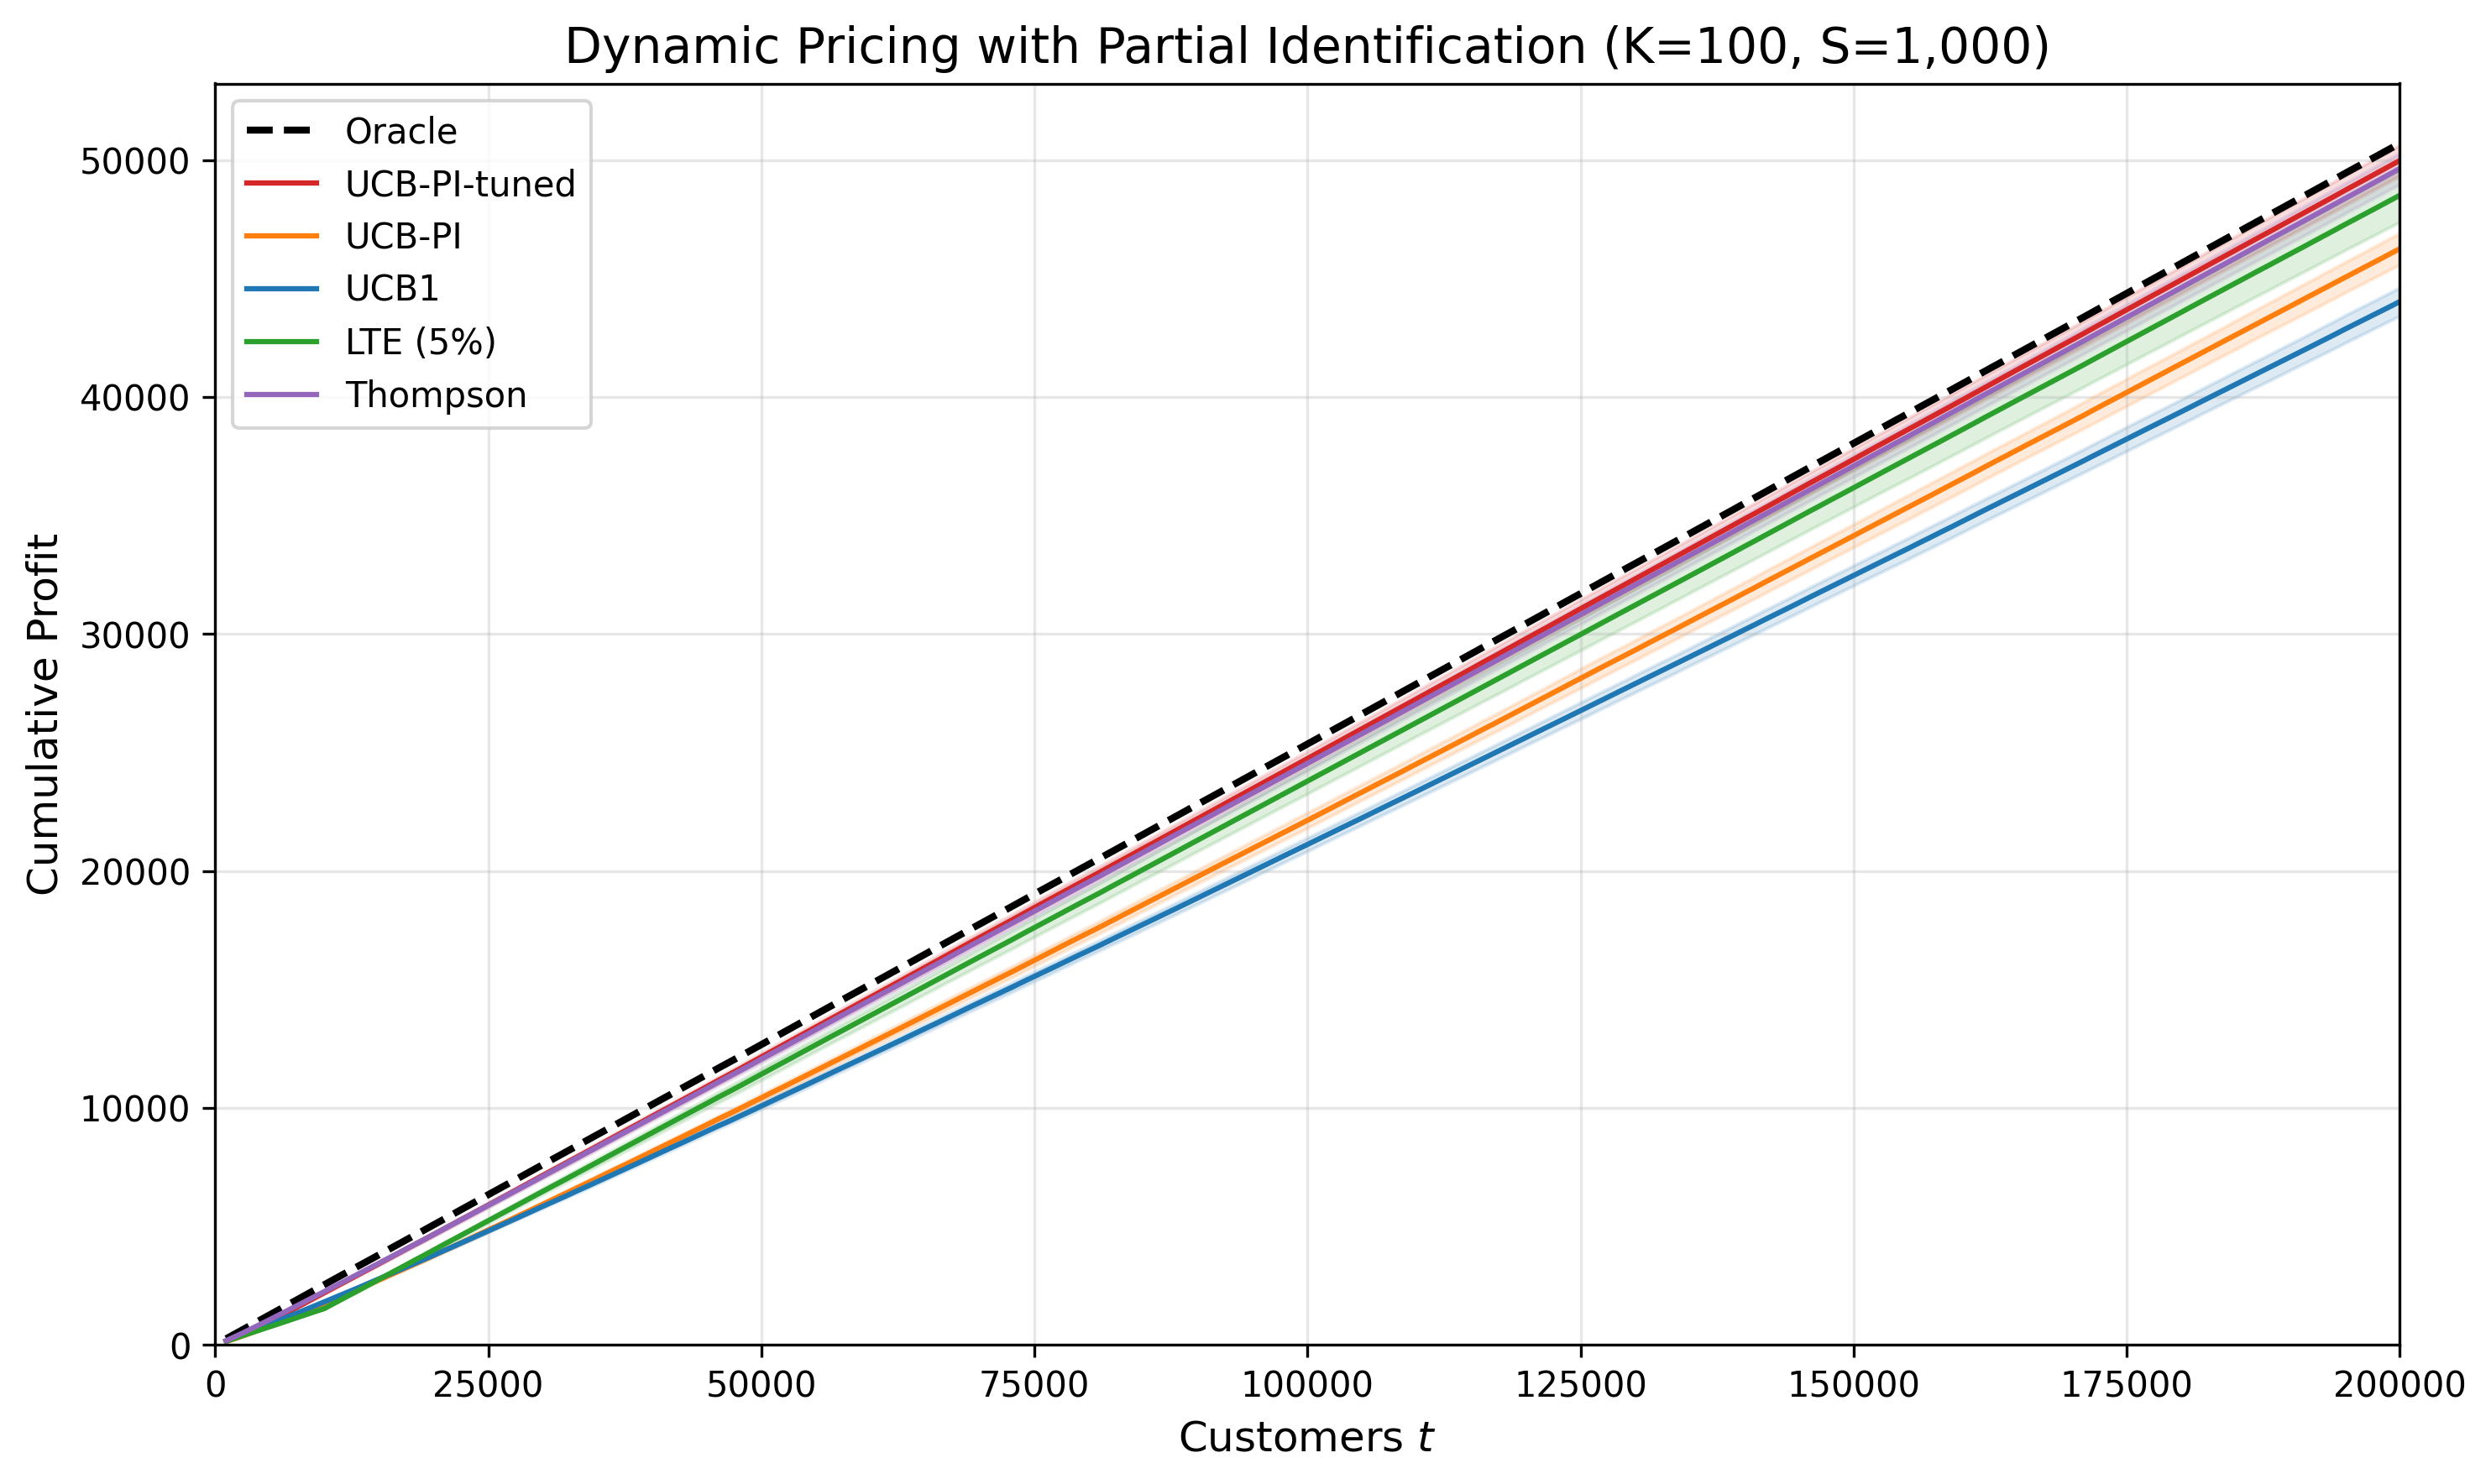
\includegraphics[width=0.9\textwidth]{../ch07_bandits/sims/structural_pricing_misra_profit.png}
\caption{Cumulative profit for dynamic pricing with partial identification. Oracle (dashed black) knows demand perfectly. Shaded regions show $\pm 2$ standard errors across 10 seeds.}
\label{fig:bandit_profit}
\end{figure}
